\usepackage{dsfont}
\usepackage{stmaryrd}
\usepackage{colortbl}
\usepackage{hyperref}

\usepackage{amsmath}
\usepackage{amssymb}

\usepackage{textcomp}

% Packages
\usepackage[pdf]{graphviz}
\usepackage{mathrsfs}

\newcommand*\circled[1]{\tikz[baseline=-0.1cm]{
    \node[shape=circle,draw,inner sep=0.48pt] (char) {\fontsize{7}{12}\textsf{#1}};}}

\DeclareMathAlphabet{\mathcal}{OMS}{cmsy}{m}{n}
\usepackage{cancel}
\newcommand\ccancel[2][red]{\renewcommand\CancelColor{\color{#1}}\cancel{#2}}
\newcommand{\nDownarrow}{\ensuremath{\text{ }\cancel{\Downarrow}\text{ }}}
\usepackage{centernot}

\usepackage{pgfplots, pgfplotstable}
\pgfplotsset{compat=1.7}
\usepgfplotslibrary{fillbetween}
\usetikzlibrary{patterns}
\pgfmathdeclarefunction{gauss}{2}{\pgfmathparse{1/(#2*sqrt(2*pi))*exp(-((x-#1)^2)/(2*#2^2))}}
\pgfmathdeclarefunction{nil}{1}{\pgfmathparse{0.001}}

\usepackage{arydshln}
\usepackage{adjustbox}
\usepackage{enumerate}
\usepackage{tikz-cd}
\usetikzlibrary{calc}
\usepackage{amsfonts}
%\usepackage{prooftrees}
\usepackage{bussproofs}
\renewcommand{\sectionautorefname}{\S}
\renewcommand{\subsectionautorefname}{\S}
\usepackage{float}

\usepackage{tikz-3dplot}
\usetikzlibrary{3d}
\usetikzlibrary{calligraphy}
\newif\ifshowcellnumber
\showcellnumbertrue

\usepackage{algorithm}
\usepackage{algpseudocode}
\usepackage{algorithmicx}
\usepackage{sourcecodepro}
\usepackage{tikz-qtree}
\usepackage{amsthm}
\usepackage{bm}
\usetikzlibrary{bayesnet}
\usetikzlibrary{arrows}
\usepackage{subcaption}
\usetikzlibrary{backgrounds}
\usetikzlibrary{tikzmark}

\newcommand{\E}{\mathbb{E}}
\newcommand{\Var}{\mathrm{Var}}
\newcommand{\Cov}{\mathrm{Cov}}

\newcommand{\CompOrder}{\mathcal{O}}
\def\graphspace{\mathbf{G}}
\def\Uniform{\mbox{\rm Uniform}}
\def\Gaussian{\mbox{\rm Gaussian}}
\def\Bernoulli{\mbox{\rm Bernoulli}}
\def\Dirichlet{\mbox{\rm Dirichlet}}

\usepackage{mathtools}% superior to amsmath
\usepackage{tikz}
% Packages
\usepackage{listings}
\DeclareRobustCommand{\hlred}[1]{{\sethlcolor{pink}\hl{#1}}}
\usepackage{fontspec}

\setmonofont[Scale=0.8]{JetBrainsMono}[
    Contextuals={Alternate},
    Path=./font/,
    Extension = .ttf,
    UprightFont=*-Regular,
    BoldFont=*-Bold,
    ItalicFont=*-Italic,
    BoldItalicFont=*-BoldItalic
]

\usepackage[skins,breakable,listings]{tcolorbox}

\usepackage[dvipsnames, table]{xcolor}
\lstdefinelanguage{kotlin}{
    comment=[l]{//},
    commentstyle={\color{gray}\ttfamily},
    emph={delegate, filter, firstOrNull, forEach, it, lazy, mapNotNull, println, repeat, assert, with, head, tail, len, return@},
    numberstyle=\noncopyable,
    identifierstyle=\color{black},
    keywords={abstract, actual, as, as?, break, by, class, companion, continue, data, do, dynamic, else, enum, expect, false, final, for, fun, get, if, import, in, infix, interface, internal, is, null, object, open, operator, override, package, private, public, return, sealed, set, super, suspend, this, throw, true, try, catch, typealias, val, var, vararg, when, where, while, tailrec, reified},
    keywordstyle={\bfseries},
    morecomment=[s]{/*}{*/},
    morestring=[b]",
    morestring=[s]{"""*}{*"""},
    ndkeywords={@Deprecated, @JvmField, @JvmName, @JvmOverloads, @JvmStatic, @JvmSynthetic, Array, Byte, Double, Float, Boolean, Int, Integer, Iterable, Long, Runnable, Short, String, int},
    ndkeywordstyle={\bfseries},
    sensitive=true,
    stringstyle={\ttfamily},
    literate={`}{{\char0}}1,
    escapeinside={(*@}{@*)}
}
\lstdefinelanguage{tidy}{
    comment=[l]{//},
    commentstyle={\color{gray}\ttfamily},
    emph={|, ->, ---, &&&},
    emphstyle={\color{red}},
    identifierstyle=\color{black},
    keywords={\|, ->, ---,&&&},
    otherkeywords={|,->,---,&&&},
    morekeywords={|,->,---,&&&},
    keywordstyle={\color{blue}\bfseries},
    morecomment=[s]{/*}{*/},
    morestring=[b]",
    morestring=[s]{"""*}{*"""},
    ndkeywords={@Deprecated, @JvmField, @JvmName, @JvmOverloads, @JvmStatic, @JvmSynthetic, Array, Byte, Double, Bool, Float, Int, Integer, Iterable, Long, Runnable, Short, String},
    ndkeywordstyle={\color{orange}\bfseries},
    sensitive=true,
    stringstyle={\color{green}\ttfamily},
    literate={`}{{\char0}}1
}

%%%%%%%%%%%%%%%%%%%%%%%%%%%%%%%%%%%%%%%%%%%
%
% Color boxes
%
%%%%%%%%%%%%%%%%%%%%%%%%%%%%%%%%%%%%%%%%%%%

\tcbset{
    enhanced jigsaw,
    breakable,
    listing only,
    boxsep=-1pt,
    top=-1pt,
    bottom=-0.5pt,
    right=-0.5pt,
    overlay first={
        \node[black!50] (S) at (frame.south) {\Large\ding{34}};
        \draw[dashed,black!50] (frame.south west) -- (S) -- (frame.south east);
    },
    overlay middle={
        \node[black!50] (S) at (frame.south) {\Large\ding{34}};
        \draw[dashed,black!50] (frame.south west) -- (S) -- (frame.south east);
        \node[black!50] (S) at (frame.north) {\Large\ding{34}};
        \draw[dashed,black!50] (frame.north west) -- (S) -- (frame.north east);
    },
    overlay last={
        \node[black!50] (S) at (frame.north) {\Large\ding{34}};
        \draw[dashed,black!50] (frame.north west) -- (S) -- (frame.north east);
    },
    before={\par\vspace{5pt}},
    after={\par\vspace{\parskip}\noindent}
}

\definecolor{slightgray}{rgb}{0.90, 0.90, 0.90}

\usepackage{soul}
\makeatletter
\def\SOUL@hlpreamble{%
    \setul{}{3.0ex}%
    \let\SOUL@stcolor\SOUL@hlcolor%
    \SOUL@stpreamble%
}
\makeatother

\newcommand{\inline}[1]{%
    \begingroup%
    \sethlcolor{slightgray}%
    \hl{\ttfamily\footnotesize #1}%
    \endgroup
}

\newcommand{\tinline}[1]{%
    \begingroup%
    \sethlcolor{slightgray}%
    \hl{\ttfamily\tiny #1}%
    \endgroup
}

\newtcblisting{halftidyinput}[1][]{%
    left skip=0.7cm,
    width=6cm,
%  left=-0.01cm,
    top=-0.1cm,
    bottom=-0.35cm,
    listing options={
        language=tidy,
        basicstyle=\ttfamily\small,
%numberstyle=\footnotesize,
        showstringspaces=false,
        tabsize=2,
        breaklines=true,
        numbers=none,
        inputencoding=utf8,
        escapeinside={(*@}{@*)},
        #1
    },
    underlay unbroken and first={%
        \path[draw=none] (interior.north west) rectangle node[white]{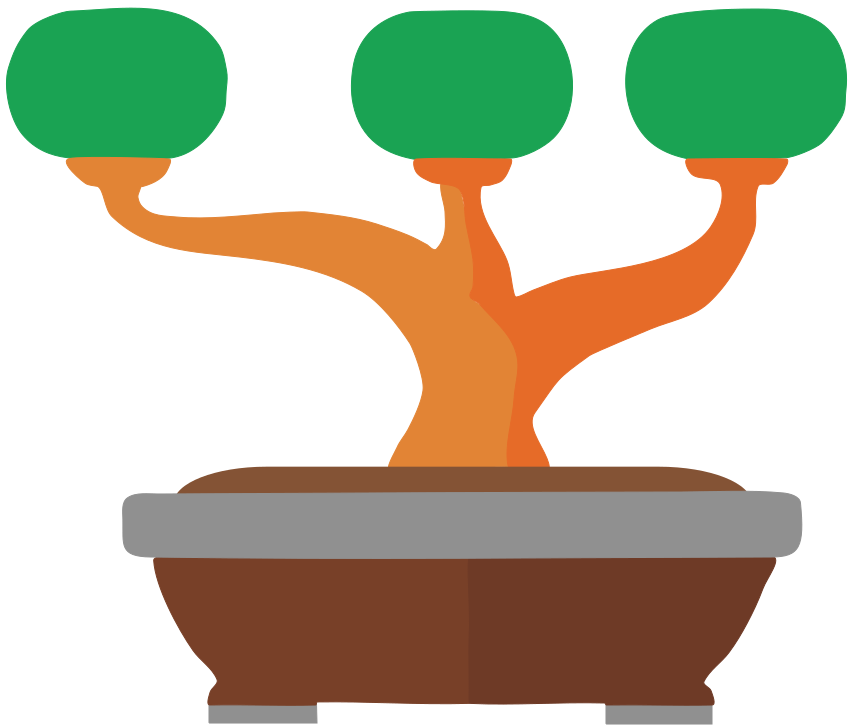
\includegraphics[width=4mm]{../figures/tidyparse_logo.png}} ([xshift=-10mm,yshift=-7mm]interior.north west);
    }
}

\newtcblisting{tidyinput}[1][]{%
    width=8.5cm,
    left=10pt,
    top=1pt,
    boxrule=1pt,
    listing options={
        language=tidy,
        basicstyle=\ttfamily\small,
%numberstyle=\footnotesize,
        showstringspaces=false,
        tabsize=2,
        breaklines=true,
        numbers=none,
        inputencoding=utf8,
        escapeinside={(*@}{@*)},
        #1
    },
    underlay unbroken and first={%
        \path[draw=none] (interior.north west) rectangle node[white]{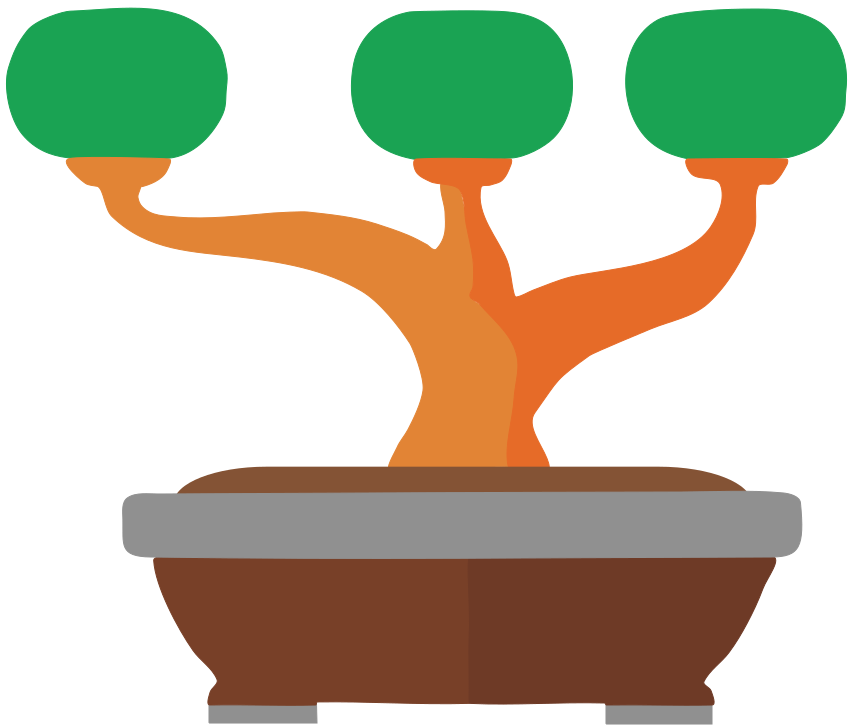
\includegraphics[width=4mm]{../figures/tidyparse_logo.png}} ([xshift=-10mm,yshift=-7mm]interior.north west);
    }
}

\newtcblisting{tidyoutput}[1][]{%
    width=8.5cm,
    left=10pt,
    top=1pt,
    boxrule=1pt,
    listing options={
        basicstyle=\ttfamily\small,
%numberstyle=\footnotesize,
        showstringspaces=false,
        tabsize=2,
        breaklines=true,
        numbers=none,
        inputencoding=utf8,
        escapeinside={(*@}{@*)},
        #1
    }
}

\lstdefinelanguage{Kotlin}{
    basicstyle = \footnotesize\ttfamily,
    comment=[l]{//},
    commentstyle={\color{gray}\ttfamily},
    emph={delegate, filter, lazy, println, return@, K, E, X, P, G, E, V},
    emphstyle={\color{red}},
    identifierstyle=\color{black},
    keywords={abstract, actual, as, as?, break, by, class, companion, continue, data, do, dynamic, else, enum, expect, false, final, for, fun, get, if, import, in, infix, interface, internal, is, null, object, operator, override, package, private, public, return, sealed, set, super, suspend, this, throw, true, try, typealias, tailrec, val, var, vararg, when, where, while},
    keywordstyle={\color{blue}\bfseries},
    morecomment=[s]{/*}{*/},
    morestring=[b]",
    morestring=[s]{"""*}{*"""},
    ndkeywords={@Deprecated, @JvmField, @JvmName, @JvmOverloads, @JvmStatic, @JvmSynthetic, Array, Byte, Double, Float, Int, Integer, Iterable, Long, Runnable, Short, String, Bool, Boolean},
    ndkeywordstyle={\color{orange}\bfseries},
    sensitive=true,
    stringstyle={\color{green}\ttfamily},
    showstringspaces=false,
    escapechar=@
}


\definecolor{A}{RGB}{6,150,104}
\definecolor{B}{RGB}{196,74,137}
\definecolor{C}{RGB}{117,237,133}
\definecolor{D}{RGB}{246,46,243}
\definecolor{E}{RGB}{89,162,12}
\definecolor{F}{RGB}{113,12,158}
\definecolor{G}{RGB}{191,205,142}
\definecolor{H}{RGB}{51,58,158}
\definecolor{I}{RGB}{244,212,3}
\definecolor{J}{RGB}{37,36,249}
\definecolor{K}{RGB}{253,165,71}
\definecolor{L}{RGB}{27,81,29}
\colorlet{LA}{A!30}
\colorlet{LB}{B!30}
\colorlet{LC}{C!30}
\colorlet{LD}{D!30}
\colorlet{LE}{E!30}
\colorlet{LF}{F!30}
\colorlet{LG}{G!30}
\colorlet{LH}{H!30}
\colorlet{LI}{I!30}
\colorlet{LJ}{J!30}
\colorlet{LK}{K!30}
\colorlet{LL}{L!30}
\newcommand{\hiliA}[1]{%
    \colorbox{LA}{$#1$}}
\newcommand{\hiliB}[1]{%
    \colorbox{LB}{$#1$}}
\newcommand{\hiliC}[1]{%
    \colorbox{LC}{$#1$}}
\newcommand{\hiliD}[1]{%
    \colorbox{LD}{$#1$}}
\newcommand{\hiliE}[1]{%
    \colorbox{LE}{$#1$}}
\newcommand{\hiliF}[1]{%
    \colorbox{LF}{$#1$}}
\newcommand{\hiliG}[1]{%
    \colorbox{LG}{$#1$}}
\newcommand{\hiliH}[1]{%
    \colorbox{LH}{$#1$}}
\newcommand{\hiliI}[1]{%
    \colorbox{LI}{$#1$}}
\newcommand{\hiliJ}[1]{%
    \colorbox{LJ}{$#1$}}
\newcommand{\hiliK}[1]{%
    \colorbox{LK}{$#1$}}
\newcommand{\hiliL}[1]{%
    \colorbox{LL}{$#1$}}
\newcommand{\highlight}[1]{%
    \colorbox{lgray}{$#1$}}
\colorlet{lred}{red!30}
\colorlet{lorange}{orange!30}
\colorlet{lgreen}{green!30}
\colorlet{lgray}{black!15}
\colorlet{dgray}{black!75}
\DeclareRobustCommand{\hlred}[1]{{\sethlcolor{lred}\hl{#1}}}
\DeclareRobustCommand{\hlorange}[1]{{\sethlcolor{lorange}\hl{#1}}}
\DeclareRobustCommand{\hlgreen}[1]{{\sethlcolor{lgreen}\hl{#1}}}
\DeclareRobustCommand{\hlgray}[1]{{\sethlcolor{lgray}\hl{#1}}}
\DeclareRobustCommand{\caret}[1]{{\sethlcolor{dgray}\textcolor{white}{\hl{#1}}}}

\usepackage{url}
\usepackage{qtree}

\usepackage{filecontents}
\usepackage{pstricks-add}
\usepackage{emoji}
\usepackage{alltt}
\usepackage{nicematrix}
\usepackage{graphicx}
\usepackage{ulem}
\usepackage{upquote}
\tikzstyle{every picture}+=[remember picture]
\usepackage{menukeys}
\pgfplotstableread[col sep=comma,]{timings_loc.csv}\loctimings
\pgfplotstableread[col sep=comma,]{timings_unloc.csv}\unloctimings
\pgfplotstableread[col sep=comma,]{natural_errors.csv}\naturalerrors
\pgfplotstableread[col sep=comma,]{synthetic_errors.csv}\syntheticerrors

\makeatletter
\DeclareRobustCommand{\cev}[1]{%
        {\mathpalette\do@cev{#1}}%
}
\newcommand{\do@cev}[2]{%
    \vbox{\offinterlineskip
    \sbox\z@{$\m@th#1 x$}%
    \ialign{##\cr
    \hidewidth\reflectbox{$\m@th#1\vec{}\mkern4mu$}\hidewidth\cr
    \noalign{\kern-\ht\z@}
        $\m@th#1#2$\cr
    }%
    }%
}
\makeatother

\makeatletter
\DeclareRobustCommand{\pder}[1]{%
    \@ifnextchar\bgroup{\@pder{#1}}{\@pder{}{#1}}}
\newcommand{\@pder}[2]{\frac{\partial#1}{\partial#2}}
\makeatother

\newcommand{\shup}{\shortuparrow}
\newcommand{\shri}{\shortrightarrow}
\newcommand{\shur}{\shup\hspace{-5pt}\shri}

\makeatletter
\def\squiggly{\bgroup \markoverwith{\textcolor{red}{\lower3\p@\hbox{\sixly \char58}}}\ULon}
\makeatother

\newcommand{\err}[1]{\smash{\squiggly{#1}{}}}
\newcommand{\stirlingii}{\genfrac{\{}{\}}{0pt}{}}

\usepgfplotslibrary{fillbetween}
\usetikzlibrary{patterns}
\pgfmathdeclarefunction{gauss}{2}{\pgfmathparse{1/(#2*sqrt(2*pi))*exp(-((x-#1)^2)/(2*#2^2))}}
\pgfmathdeclarefunction{nil}{1}{\pgfmathparse{0.001}}

\usepackage[symbol,hang,flushmargin]{footmisc}

\renewcommand{\thefootnote}{\fnsymbol{footnote}}

\newcommand{\nobarfrac}{\genfrac{}{}{0pt}{}}

\newcommand{\mkTrellis}[1]{
  \begin{tikzpicture}
    \def\dx{20pt}
    \def\dy{30pt}
    \newcounter{i}
    \stepcounter{i}
    \node[circle, draw, fill=black!30] (\arabic{i}) at (0,0){};
    \foreach [count=\i] \x in {2,...,#1}{
      \pgfmathsetmacro{\lox}{\x-1}%
      \pgfmathsetmacro{\loxt}{\x-3}%
      \foreach [count=\j] \xx in {-\lox,-\loxt,...,\lox}{
        \pgfmathsetmacro{\jj}{\j-1}%
        \stepcounter{i}
        \pgfmathsetmacro{\kk}{\xx-2}%
        \pgfmathsetmacro{\lbl}{\lox!/(\jj!*(\lox-\jj)!)}
        \ifnum\x<\kk
            \pgfmath\node[circle, draw]  (\arabic{i}) at (\xx*\dx, -\lox*\dy) {};
        \else
            \pgfmath\node[circle, draw, fill=black!30]  (\arabic{i}) at (\xx*\dx, -\lox*\dy) {};
        \fi
      }
    }
    \newcounter{z}
    \newcounter{xn}
    \newcounter{xnn}
    \pgfmathsetmacro{\maxx}{#1 - 1}
    \foreach \x in {1,...,\maxx}{
      \foreach \xx in {1,...,\x}{
        \stepcounter{z}
        \setcounter{xn}{\arabic{z}}
        \addtocounter{xn}{\x}
        \setcounter{xnn}{\arabic{xn}}
        \stepcounter{xnn}
        \draw [<-] (\arabic{z}) -- (\arabic{xn});
        \draw [<-] (\arabic{z}) -- (\arabic{xnn});
      }
    }
  \end{tikzpicture}
}

\newcommand{\dx}{20pt}
\newcommand{\dy}{30pt}
\newcounter{i}
\newcounter{z}
\newcounter{xn}
\newcounter{xnn}
\newcommand{\mkTrellisAppend}[1]{
    \begin{tikzpicture}
        \setcounter{i}{0}
        \setcounter{z}{0}
        \setcounter{xn}{0}
        \setcounter{xnn}{0}
        \stepcounter{i}
        \node[circle, draw] (\arabic{i}) at (0,0){};
        \foreach [count=\i] \x in {2,...,#1}{
            \pgfmathsetmacro{\lox}{\x-1}%
            \pgfmathsetmacro{\loxt}{\x-3}%
            \foreach [count=\j] \xx in {-\lox,-\loxt,...,\lox}{
                \pgfmathsetmacro{\jj}{\j-1}%
                \stepcounter{i}
                \pgfmathsetmacro{\kk}{\xx+2}%
                \pgfmathsetmacro{\lbl}{\lox!/(\jj!*(\lox-\jj)!)}
                \ifnum\x>\kk
                \pgfmath\node[circle, draw, fill=black!30]  (\arabic{i}) at (\xx*\dx, -\lox*\dy) {};
                \else
                \pgfmath\node[circle, draw]  (\arabic{i}) at (\xx*\dx, -\lox*\dy) {};
                \fi
            }
        }
        \pgfmathsetmacro{\maxx}{#1 - 1}
        \foreach \x in {1,...,\maxx}{
            \foreach \xx in {1,...,\x}{
                \stepcounter{z}
                \setcounter{xn}{\arabic{z}}
                \addtocounter{xn}{\x}
                \setcounter{xnn}{\arabic{xn}}
                \stepcounter{xnn}
                \draw [<-] (\arabic{z}) -- (\arabic{xn});
                \draw [<-] (\arabic{z}) -- (\arabic{xnn});
            }
        }
    \end{tikzpicture}
}

\newcommand{\mkTrellisInsert}[1]{
    \begin{tikzpicture}
        \setcounter{i}{0}
        \setcounter{z}{0}
        \setcounter{xn}{0}
        \setcounter{xnn}{0}
        \stepcounter{i}
        \node[circle, draw] (\arabic{i}) at (0,0){};
        \foreach [count=\i] \x in {2,...,#1}{
            \pgfmathsetmacro{\lox}{\x-1}%
            \pgfmathsetmacro{\loxt}{\x-3}%
            \foreach [count=\j] \xx in {-\lox,-\loxt,...,\lox}{
                \pgfmathsetmacro{\jj}{\j-1}%
                \stepcounter{i}
                \pgfmathsetmacro{\mp}{\xx+#1}%
                \pgfmathsetmacro{\mq}{\xx+\x}%
                \pgfmathsetmacro{\lbl}{\lox!/(\jj!*(\lox-\jj)!)}
                \ifnum\x>\mp
                \pgfmath\node[circle, draw, fill=black!30]  (\arabic{i}) at (\xx*\dx, -\lox*\dy) {};
                \else
                \ifnum#1<\mq
                \pgfmath\node[circle, draw, fill=black!30]  (\arabic{i}) at (\xx*\dx, -\lox*\dy) {};
                \else
                \pgfmath\node[circle, draw]  (\arabic{i}) at (\xx*\dx, -\lox*\dy) {};
                \fi
                \fi

            }
        }
        \pgfmathsetmacro{\maxx}{#1 - 1}
        \foreach \x in {1,...,\maxx}{
            \foreach \xx in {1,...,\x}{
                \stepcounter{z}
                \setcounter{xn}{\arabic{z}}
                \addtocounter{xn}{\x}
                \setcounter{xnn}{\arabic{xn}}
                \stepcounter{xnn}
                \draw [<-] (\arabic{z}) -- (\arabic{xn});
                \draw [<-] (\arabic{z}) -- (\arabic{xnn});
            }
        }
    \end{tikzpicture}
}

\usetikzlibrary{automata, positioning, arrows}
\tikzset{
    node distance=3cm, % specifies the minimum distance between two nodes. Change if necessary.
%    every state/.style={thick, fill=gray!10}, % sets the properties for each ’state’ node
    initial text=$ $, % sets the text that appears on the start arrow
}
\newcommand*{\ttinline}[1]{{\sethlcolor{slightgray}\ttfamily\footnotesize\relax\highlight{#1}}}